\chapter{Robot Control}
The robot is required to move to any point inside the image frame by controlling the wheels speed. This goal can be achieved by designing a controller to correct for position errors sensed by the camera. To design the controller, the knowledge of the robot's motion is extremely important. The kinematics model of the robot was discussed in section \ref{robot_modelling} as it is used in this section. \\
In literature, the commands for the system (controller output) are usually the linear velocity $v_c$ and the angular velocity $\omega_c$. First, a relationship between the controller output and the wheels’ motor angular velocity is needed. Solving for the motors’ angular velocities gives the following:

\begin{equation}
    \omega_r = \frac{1}{R_w} (v_c + \frac{D}{2}\omega_c)
\end{equation}
\begin{equation}
    \omega_l = \frac{1}{R_w} (v_c - \frac{D}{2}\omega_c)
\end{equation}

Where $R_w$ is the wheel radius. These are called the inverse kinematic equations.\\
The trajectory is described by a path planning algorithm. This trajectory is broken down into single points (x and y coordinates) to be followed by the robot. Therefore, the controller must bring the robot to these points that are calculated in real time. The design of this controller is described by the block diagram in Figure \ref{block_diagram}.

\begin{figure}[thb]
    \centering
    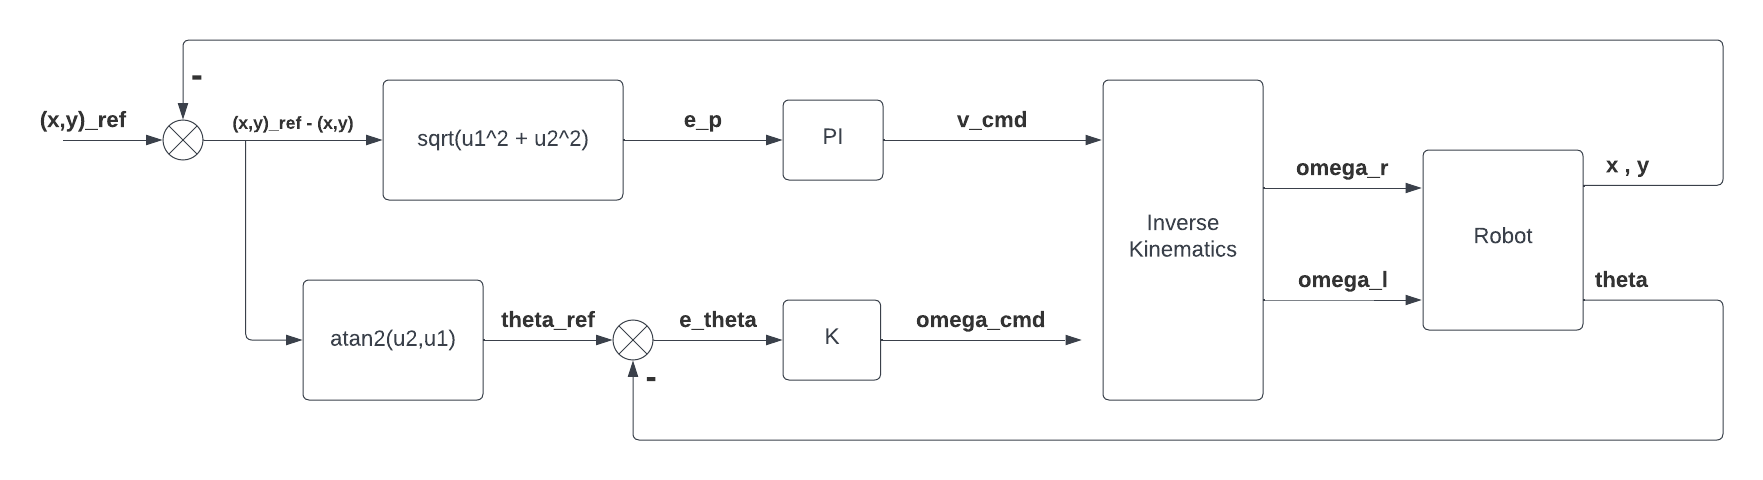
\includegraphics[width=1\textwidth]{images/Block_diagram.png}
    \caption{Controller block diagram}\label{block_diagram}
\end{figure}

The reference (x,y) coordinates are given by the path planning algorithm. These coordinates are compared to the position measured by the image processing algorithm to compute an error. The errors are described as:
\begin{equation}
    e_p = \sqrt{(x_{ref} - x)^2+(y_{ref} - y)^2}
\end{equation}
\begin{equation}
    e_{\theta} = \theta_{ref} - \theta 
\end{equation}
\begin{equation}
    \theta_{ref} = atan2\left(\frac{y_{ref}-y}{x_{ref} - x}\right)
\end{equation}

There is an error of the distance between the desired point and our measured point, and there is another error that calculates the difference between the robot’s orientation and the angle between the robot’s x-axis and the distance vector. The first error helps the robot to approach the desired coordinate as best as possible and the second error orients the robot towards the desired coordinates. The position error is fed to a PI controller and the orientation error is fed to a proportional controller to generate the following commands:
\begin{equation}
    v_{cmd} = k_p e_p + k_i \int e_p dt 
\end{equation}
\begin{equation}
    \omega_{cmd} = k_p e_{\theta}
\end{equation}

The controller gains were tuned for best performance. The robot was tested with multiple reference locations to measure the step response. Some of these results are shown in Figure \ref{robot_resp}. Large distances were input to the robot model to check if there was still a fast response. Most of the time the robot operates with the maximum speed which ensures that the robot moves as fast as possible. It is expected to have a similar speed response for shorter distances.

\begin{figure}[thb]
    \centering
    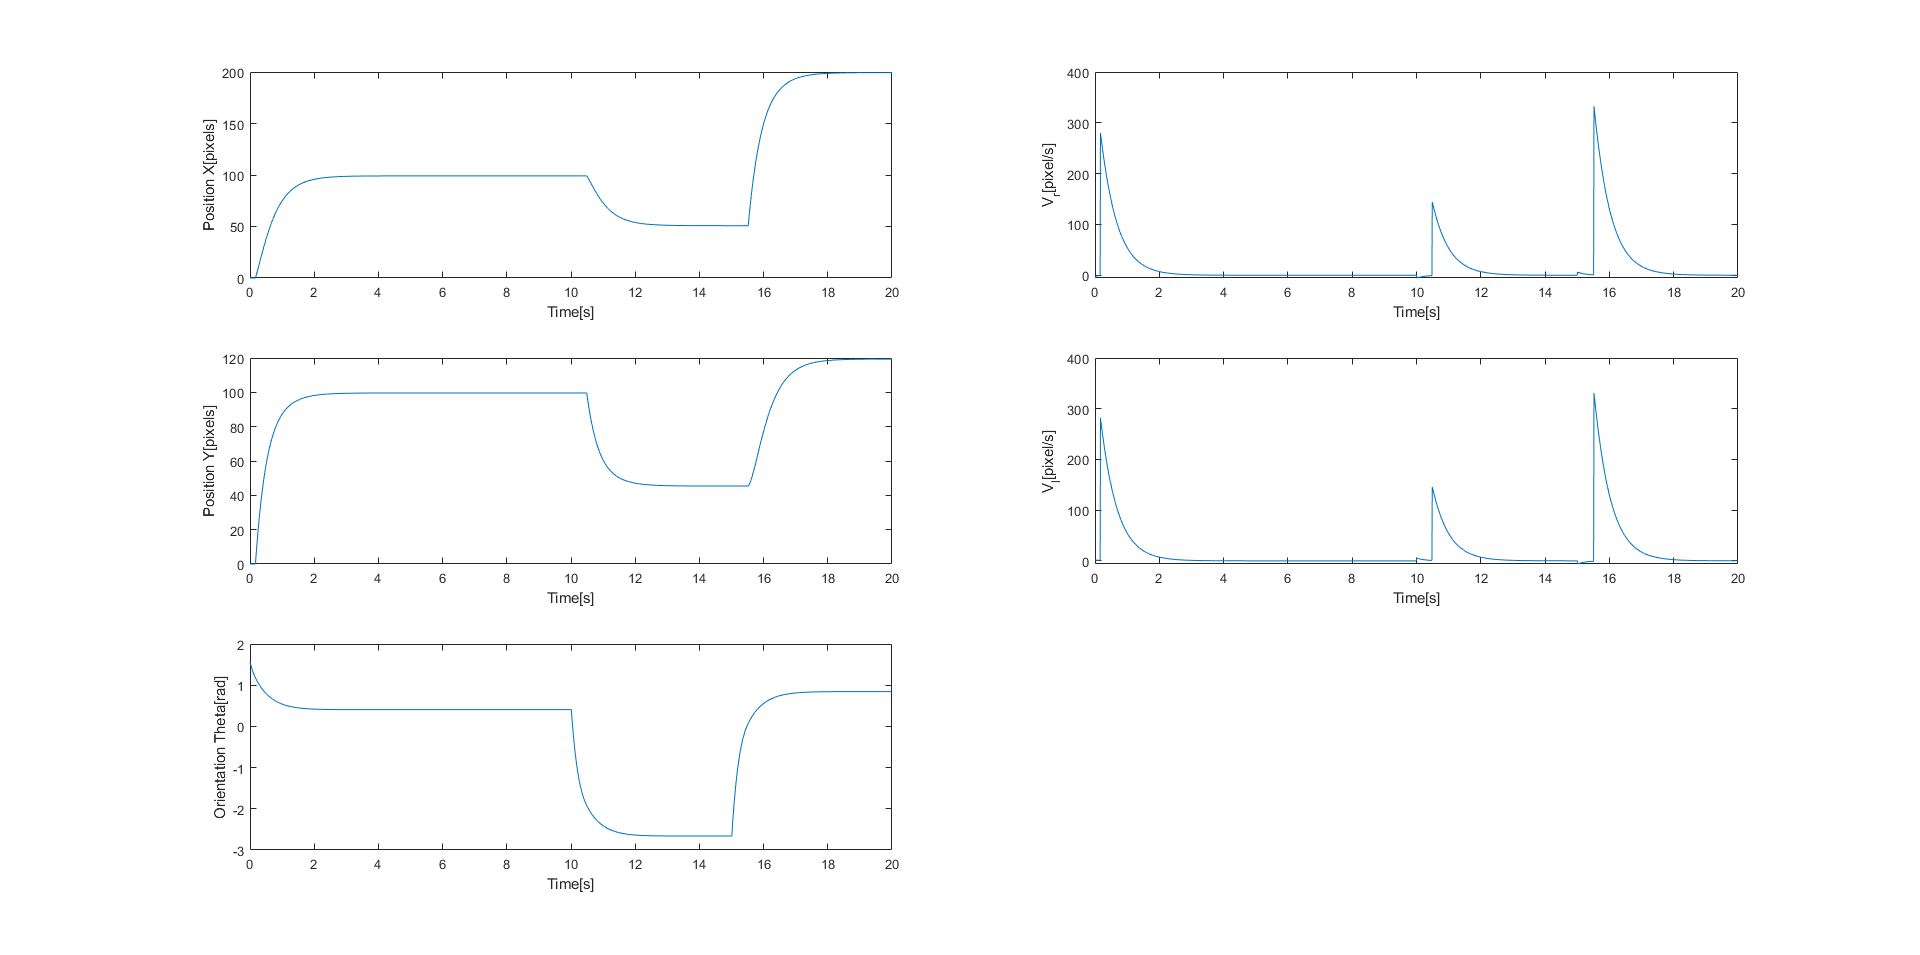
\includegraphics[width=0.6\textwidth]{images/robot_response.png}
    \caption{Robot response to multiple reference positions}\label{robot_resp}
\end{figure}